%%%%%%%%%%%%%%%%%%%%%%%%%%%%%%%%%%%%%
%                                   %
% Compile with XeLaTeX and biber    %
%                                   %
% Questions or comments:            %
%                                   %
% joshua dot mcneill at uga dot edu %
%                                   %
%%%%%%%%%%%%%%%%%%%%%%%%%%%%%%%%%%%%%

\documentclass{beamer}
  % Read in standard preamble (cosmetic stuff)
  %%%%%%%%%%%%%%%%%%%%%%%%%%%%%%%%%%%%%%%%%%%%%%%%%%%%%%%%%%%%%%%%
% This is a standard preamble used in for all slide documents. %
% It basically contains cosmetic settings.                     %
%                                                              %
% Joshua McNeill                                               %
% joshua dot mcneill at uga dot edu                            %
%%%%%%%%%%%%%%%%%%%%%%%%%%%%%%%%%%%%%%%%%%%%%%%%%%%%%%%%%%%%%%%%

% Beamer settings
% \usetheme{Berkeley}
\usetheme{CambridgeUS}
% \usecolortheme{dove}
% \usecolortheme{rose}
\usecolortheme{seagull}
\usefonttheme{professionalfonts}
\usefonttheme{serif}
\setbeamertemplate{bibliography item}{}

% Packages and settings
\usepackage{fontspec}
  \setmainfont{Charis SIL}
\usepackage{hyperref}
  \hypersetup{colorlinks=true,
              allcolors=blue}
\usepackage{graphicx}
  \graphicspath{{../../figures/}}
\usepackage[normalem]{ulem}
\usepackage{enumerate}

% Document information
\author{M. McNeill}
\title[FREN2001]{Français 2001}
\institute{\url{joshua.mcneill@uga.edu}}
\date{}

%% Custom commands
% Lexical items
\newcommand{\lexi}[1]{\textit{#1}}
% Gloss
\newcommand{\gloss}[1]{`#1'}
\newcommand{\tinygloss}[1]{{\tiny`#1'}}
% Orthographic representations
\newcommand{\orth}[1]{$\langle$#1$\rangle$}
% Utterances (pragmatics)
\newcommand{\uttr}[1]{`#1'}
% Sentences (pragmatics)
\newcommand{\sent}[1]{\textit{#1}}
% Base dir for definitions
\newcommand{\defs}{../definitions}


  % Packages and settings

  % Document information
  \subtitle[Loisirs (jouer) et prépositions]{Les loisirs que nous jouons et \lexi{à} et \lexi{de}}

\begin{document}
  % Read in the standard intro slides (title page and table of contents)
  \begin{frame}
    \titlepage
    \tiny{Office: % Basically a variable for office hours location
Gilbert 121\\
          Office hours: % Basically a variable for office hours
 lundi, mercredi, vendredi 10:10--11:10
}
  \end{frame}

  \begin{frame}{}
    \begin{center}
      \Large Quiz
    \end{center}
  \end{frame}

  \begin{frame}{Révision du verbe}
    \begin{center}
      \begin{tabular}{l | l l | l l}
  \multicolumn{5}{c}{jouer \gloss{to play}} \\
      & \multicolumn{2}{l |}{singulier} & \multicolumn{2}{l}{pluriel} \\
  \hline
  1re & je         & joue               & nous        & jouons \\
  2e  & tu         & joues              & vous        & jouez \\
  \hline
  3e  & il (masc)  &                    & ils (masc)  & \\
      & elle (fem) & joue               & elles (fem) & jouent \\
      & on         &                    &             & \\
\end{tabular}

    \end{center}
  \end{frame}
  
  \begin{frame}{Conjugaisons \gloss{Conjugations}}
    Quelles sont les bonnes conjugaisons du verbe \lexi{jouer}? \\
    \tinygloss{What are the correct conjugations of the verb \lexi{jouer}?}
    \begin{enumerate}
      \item Je \underline{\uncover<2->{\ joue\ }} au loto.
      \item Mon colocataire \underline{\uncover<3->{\ joue\ }} du harmonica.
      \item Les Bulldogs \underline{\uncover<4->{jouent}} au football américain.
      \item Nous \underline{\uncover<5->{jouons}} au basket.
      \item Vous \underline{\uncover<6->{jouez}} de la musique classique.
    \end{enumerate}
  \end{frame}

  \begin{frame}{Contractions \gloss{Contractions}}
    Comment est-ce qu'on change la préposition? \\
    \tinygloss{How does one change the preposition?}
    \begin{enumerate}
      \item (de la) Dave Grohl joue \underline{\uncover<2->{de la}} batterie.
      \item (à les) Mes grands-parents jouent \underline{\uncover<3->{aux}} cartes.
      \item (à la) Ma cousine reste \underline{\uncover<4->{à la}} maison.
      \item (à le) Il y a beaucoup de personnes \underline{\uncover<5->{\ au\ }} concert.
      \item (de le) Est-ce que tu es \underline{\uncover<6->{\ du\ }} Canada?
      \item (de le) Non, je suis \underline{\uncover<7->{de l'}} Alabama.
      \item (à la) Nous travaillons \underline{\uncover<8->{à l'}} école.
    \end{enumerate}
  \end{frame}

  \begin{frame}{Qu'est-ce qu'ils font?}
    \begin{columns}
      \column{0.5\textwidth}
        \begin{enumerate}
          \item Loïc est sportif.
          \item<2-> Helen Gillet est musicienne.
          \item<3-> Jean-Luc Godard adore le cinéma.
          \item<4-> Maxime Vachier-Lagrave adore les jeux de société.
          \item<5-> Trombone Shorty est fanatique de jazz.
        \end{enumerate}
      \column{0.5\textwidth}
        \begin{minipage}[c][0.6\textheight]{\linewidth}
          \begin{center}
            \only<1>{
              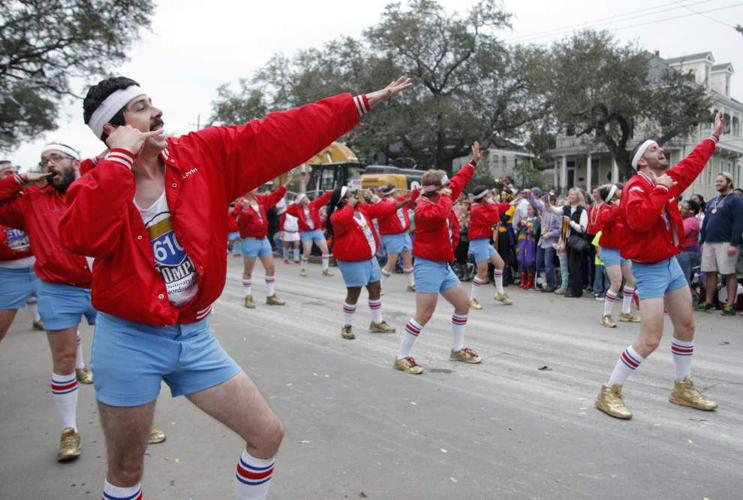
\includegraphics[scale=0.2]{stompers.jpg}
            }
            \only<2>{
              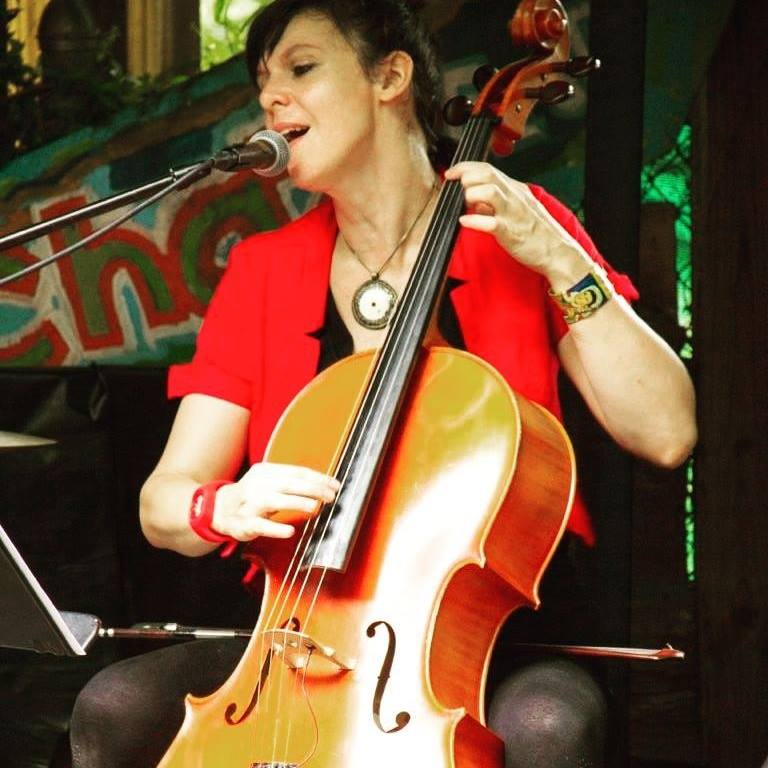
\includegraphics[scale=0.2]{helen_gillet.jpg}
            }
            \only<3>{
              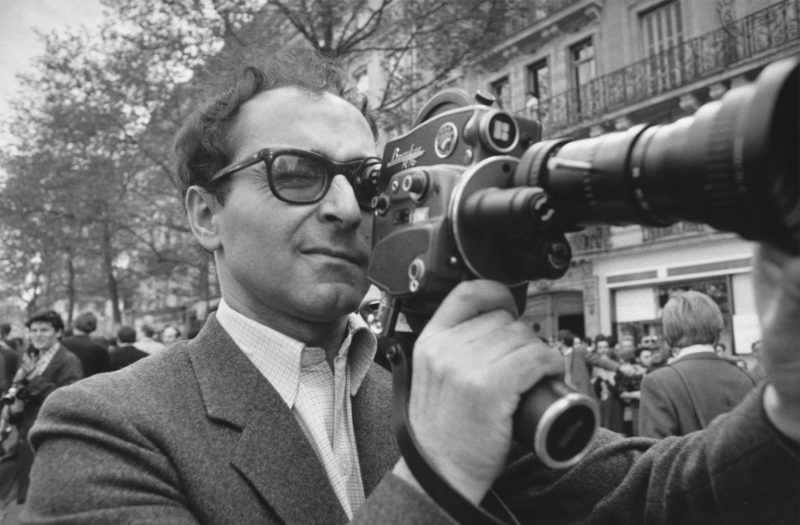
\includegraphics[scale=0.23]{godard.jpg}
            }
            \only<4>{
              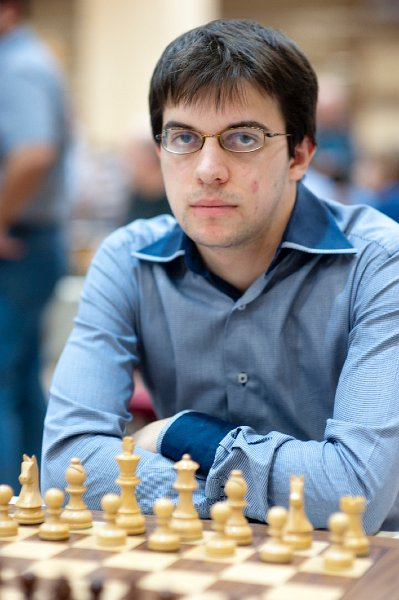
\includegraphics[scale=0.24]{maxime_vachier-lagrave.jpg}
            }
            \only<5>{
              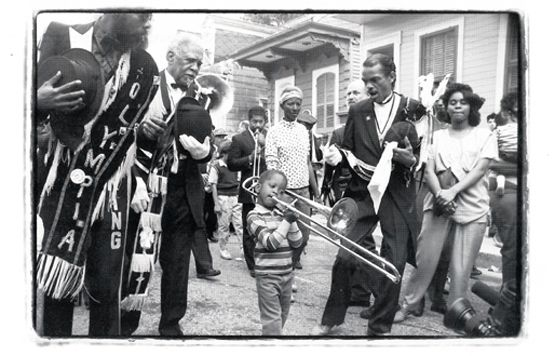
\includegraphics[scale=0.3]{trombone_shorty.jpg}
            }
          \end{center}
        \end{minipage}
    \end{columns}
  \end{frame}

  \begin{frame}{Liaisons}
    Est-ce que vous entendez une liaison?
    \begin{columns}
      \column{0.5\textwidth}
        \begin{enumerate}
          \item nous avons \underline{\uncover<2->{oui}}
          \item des colocataires \underline{\uncover<3->{non}}
          \item chez nous \underline{\uncover<4->{non}}
          \item chez elles \underline{\uncover<5->{oui}}
          \item ils arrivent \underline{\uncover<6->{oui}}
        \end{enumerate}
      \column{0.5\textwidth}
        \begin{enumerate}
          \setcounter{enumi}{5}
          \item les yeux bleus \underline{\uncover<7->{oui}}
          \item très intelligent \underline{\uncover<8->{oui}}
          \item nos copains \underline{\uncover<9->{non}}
          \item un harmonica \underline{\uncover<10->{oui}}
          \item les cheveux noirs \underline{\uncover<11->{non}}
        \end{enumerate}
    \end{columns}
  \end{frame}

  \begin{frame}{Deux vérités et un mensonge \gloss{Two truths and a lie}}
    En groupes de 3 à 5, dis deux vérités et un mensonge par rapport à toi, à tour de rôle, et fais deviner lequel est le mensonge à tes camarades de groupe. \\
    \tinygloss{In groups of 3 to 5, take turns telling two truths and one lie about yourself, and have your groupmates guess which one is the lie.} \\
    \textbf{Modèle:} \\
    \begin{description}
      \item[E1:] J'ai 20 ans, je joue au rugby et j'habite à Watkinsville.
      \item[] \tinygloss{I'm 20 years old, I play rugby, and I have two sisters.}
      \item[E2:] Est-ce que tu n'as pas 20 ans?
      \item[] \tinygloss{Are you not 20 years old?}
      \item[E1:] Si, j'ai 20 ans.
      \item[] \tinygloss{Yes I am. I am 20 years old.}
      \item[E3:] Est-ce que tu ne joues pas au rugby?
      \item[] \tinygloss{Do you not play rugby?}
      \item[E1:] Oui, c'est le mensonge!
      \item[] \tinygloss{Yes, that's the lie!}
    \end{description}
  \end{frame}

  \begin{frame}{}
    \begin{center}
      \Large Questions?
    \end{center}
  \end{frame}
\end{document}
